% =============================================================================
% COMPUTATIONAL COMPLEXITY ANALYSIS APPENDIX
% =============================================================================

\subsection{Computational Complexity Analysis}\label{sec:complexity}

We analyze the computational complexity of GSC and show it maintains the same asymptotic complexity as classical spectral clustering (SC).

\subsubsection{Theoretical Analysis}

For $N$ samples, $D$ dimensions, and $k_c$ clusters, the algorithm has three main costs:

\paragraph{1. Graph Construction.}
For point clouds, we construct a $k$-NN graph with $k = \lceil \log N \rceil$. Tree-based methods (KD-tree, Ball-tree) achieve $\mathcal{O}(DN \log N)$ in low dimensions but degrade to $\mathcal{O}(DN^2)$ when $D \gtrsim 20$~\cite{bentley1975multidimensional}. The total cost is:
\begin{equation}
    T_{\text{knn}} = c_1 \cdot DN^2
\end{equation}
where $c_1$ depends on the tree structure efficiency.

\paragraph{2. Eigendecomposition (Dominant).}
Using ARPACK~\cite{lehoucq1998arpack} on a sparse Laplacian with $\mathrm{nnz} = \mathcal{O}(Nk) = \mathcal{O}(N \log N)$ edges:
\begin{equation}
    T_{\text{eig}} = c_2 \cdot N \cdot \mathrm{nnz} = c_2 \cdot N^2 \log N
\end{equation}

\paragraph{3. GSC-Specific: Vertex Measure.}
Computing $\nu_{t,\alpha} = ([\rmP^t]^\top \mu)^{\odot \alpha}$ requires $t$ sparse matrix-vector products:
\begin{equation}
    T_{\nu} = c_3 \cdot t \cdot \mathrm{nnz} = c_3 \cdot tN \log N
\end{equation}

\paragraph{Total Complexity.}
The total runtime is:
\begin{equation}
    T(N) = c_1 DN^2 + c_2 N^2 \log N + c_3 tN \log N
\end{equation}

Asymptotically, the eigendecomposition dominates and $T(N) = \mathcal{O}(N^2 \log N)$. The GSC overhead ratio $T_\nu / T_{\text{eig}} = \mathcal{O}(t/N) \to 0$, so GSC and SC have identical asymptotic complexity.

\paragraph{Practical Consideration.}
In practice, when $D \approx \log N$ (e.g., $D = 10$, $N = 20000 \Rightarrow \log N \approx 10$), the $k$-NN term $c_1 DN^2$ competes with the eigendecomposition term $c_2 N^2 \log N$. Since the constants $c_1, c_2$ are implementation-dependent, the effective complexity becomes:
\begin{equation}
    T(N) \approx (c_1 D + c_2 \log N) \cdot N^2
\end{equation}
This explains why empirical fits to $N^2 \log N$ show slight deviations at large $N$: the $DN^2$ term contributes a non-negligible constant factor. Nevertheless, the $\mathcal{O}(N^2 \log N)$ model provides a good fit ($R^2 > 0.98$), confirming that both terms scale similarly.

\subsubsection{Experimental Validation}

We validate on two settings: point clouds (with $k$-NN construction) and networks (adjacency given).

\paragraph{Setup.}
Gaussian mixtures with $k_c = 3$ clusters, $D = 10$, $N \in \{500, \ldots, 20000\}$ for point clouds; sparse directed graphs with degree $\approx 2\log N$, $N \in \{500, \ldots, 10000\}$ for networks. GSC uses $t = 5$, $\alpha = 0.5$.

\begin{table}[h]
\centering
\caption{Goodness of fit ($R^2$) for complexity models.}
\label{tab:complexity_validation}
\begin{tabular}{l|cc|c}
\toprule
Setting & SC & GSC & Model \\
\midrule
Point clouds & 0.985 & 0.986 & $T \propto N^2 \log N$ \\
Networks & 0.983 & 0.983 & $T \propto N \cdot \mathrm{nnz}$ \\
\bottomrule
\end{tabular}
\end{table}

\begin{figure}[h]
    \centering
    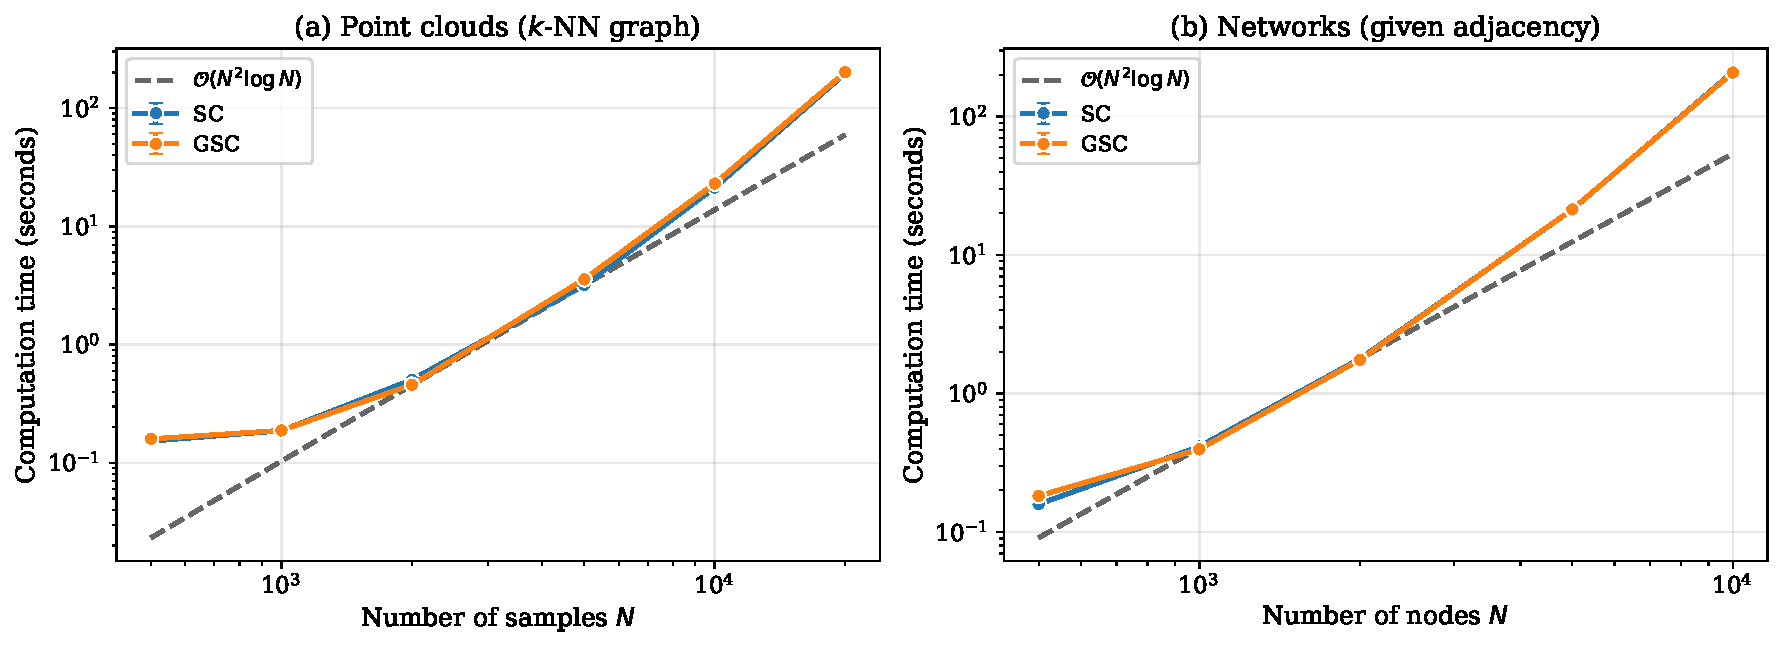
\includegraphics[width=\textwidth]{results/complexity_analysis/complexity_summary.pdf}
    \caption{Runtime comparison. Both SC and GSC follow $\mathcal{O}(N^2 \log N)$ scaling (dashed). The slight upward deviation at large $N$ reflects the $\mathcal{O}(DN^2)$ $k$-NN cost when $D \approx \log N$.}
    \label{fig:complexity_comparison}
\end{figure}

\paragraph{Results.}
Table~\ref{tab:complexity_validation} confirms $R^2 > 0.98$ for both methods. Figure~\ref{fig:complexity_comparison} shows SC and GSC timing curves are indistinguishable, with minor deviation at high $N$ due to the $k$-NN term. For networks (no $k$-NN step), the fit is tighter.

\paragraph{Networks.}
When the adjacency matrix is given, complexity reduces to $T = \mathcal{O}(N \cdot \mathrm{nnz})$: i.e., $\mathcal{O}(N^2 \log N)$ for sparse graphs, $\mathcal{O}(N^3)$ for dense.

\subsubsection{Grid Search Cost}

In practice, GSC is used with a grid search over hyperparameters $(t, \alpha)$ to optimize an internal validity measure (e.g., Calinski-Harabasz). Let $\mathcal{G} = \{(t_1, \alpha_1), \ldots, (t_{|\mathcal{G}|}, \alpha_{|\mathcal{G}|})\}$ denote the parameter grid. The total complexity becomes:
\begin{equation}
    T_{\text{grid}}(N) = |\mathcal{G}| \cdot T_{\text{single}}(N) = \mathcal{O}(|\mathcal{G}| \cdot N^2 \log N)
\end{equation}
where $T_{\text{single}}$ is the cost of a single GSC fit. This linear scaling in $|\mathcal{G}|$ is exact since each parameter evaluation is independent.

\subsubsection{Conclusion}

GSC has the same asymptotic complexity as SC: $\mathcal{O}(N^2 \log N)$ for sparse graphs. The vertex measure adds $\mathcal{O}(tN \log N)$ overhead, negligible for $N \gg t$. Grid search multiplies the cost by $|\mathcal{G}|$ but preserves the complexity class. In practice, the $k$-NN term $\mathcal{O}(DN^2)$ contributes when $D \approx \log N$, but both SC and GSC are equally affected.

% References:
% \bibitem{vonluxburg2007tutorial} U. von Luxburg. A tutorial on spectral clustering. Stat. Comput., 17(4):395--416, 2007.
% \bibitem{lehoucq1998arpack} R. Lehoucq, D. Sorensen, C. Yang. ARPACK Users' Guide. SIAM, 1998.
% \bibitem{bentley1975multidimensional} J. Bentley. Multidimensional binary search trees. CACM, 18(9):509--517, 1975.
